\let\negmedspace\undefined
\let\negthickspace\undefined
\documentclass[journal]{IEEEtran}
\usepackage[a5paper, margin=10mm, onecolumn]{geometry}
%\usepackage{lmodern} % Ensure lmodern is loaded for pdflatex
\usepackage{tfrupee} % Include tfrupee package

\setlength{\headheight}{1cm} % Set the height of the header box
\setlength{\headsep}{0mm}     % Set the distance between the header box and the top of the text

\usepackage{gvv-book}
\usepackage{gvv}
\usepackage{cite}
\usepackage{amsmath,amssymb,amsfonts,amsthm}
\usepackage{algorithmic}
\usepackage{graphicx}
\usepackage{textcomp}
\usepackage{xcolor}
\usepackage{txfonts}
\usepackage{listings}
\usepackage{enumitem}
\usepackage{mathtools}
\usepackage{gensymb}
\usepackage{comment}
\usepackage[breaklinks=true]{hyperref}
\usepackage{tkz-euclide} 
\usepackage{listings}
% \usepackage{gvv}                                        
\def\inputGnumericTable{}                                 
\usepackage[latin1]{inputenc}                                
\usepackage{color}                                            
\usepackage{array}                                            
\usepackage{longtable}                                       
\usepackage{calc}                                             
\usepackage{multirow}                                         
\usepackage{hhline}                                           
\usepackage{ifthen}                                           
\usepackage{lscape}
\begin{document}

\bibliographystyle{IEEEtran}
\vspace{3cm}

\title{NCERT-11.16.3.21.3}
\author{EE24BTECH11065 - Spoorthi yellamanchali
}
% \maketitle
% \newpage
% \bigskip
{\let\newpage\relax\maketitle}

\renewcommand{\thefigure}{\theenumi}
\renewcommand{\thetable}{\theenumi}
\setlength{\intextsep}{10pt} % Space between text and floats


\numberwithin{equation}{enumi}
\numberwithin{figure}{enumi}
\renewcommand{\thetable}{\theenumi}


\textbf{Question:}
\\
In a class of 60 students, 30 opted for $NCC$, 32 opted for $NSS$ and 24 opted for both $NCC$ and $NSS$. If one of these students is selected at random, find the probability that the student has opted for $NSS$ but not $NCC$.
\\
\textbf{Solution: }
Let us define $A$ and $B$ as shown in the table \ref{table}
\\
\begin{table}[h!]
    \centering
    
\begin{tabular}[12pt]{ |c| c|} 
    \hline
    {Event} & {Denotation}\\ 
    \hline
    $A $ &  Student do pass in English \\
    \hline 
    $ A^\prime $ & Student does not pass in English\\
    \hline
    $ B $ & Student do pass in Hindi\\
    \hline   
    $ B^\prime $ & Student does not pass in English\\
    \hline
\end{tabular}

   \label{table}
\end{table}


Then, according to the given question,

\begin{align}
    Pr\brak{A} = \frac{32}{60} = \frac{8}{15}
\end{align}
Let $B$ be the event that a student opts for $NCC$ , then 
\begin{align}
    Pr\brak{B} = \frac{30}{60} = \frac{1}{2}
\end{align}
then, $A.B$ will denote the event that a student opts for both $NSS$ and $NCC$,and,
\begin{align}
    Pr\brak{AB} = \frac{24}{60} = \frac{2}{5}
\end{align}
On using the following postulates given in table \ref{table2} and the additivity axiom, which is,
\begin{table}[h!]
    \centering
    \begin{tabular}{|l|c l|c l|}
    \hline
    & (a) & & (b) & \\
    \hline
    Postulate 2 & $A + 0 = A$ & & $A \cdot 1 = A$ & \\
    \hline
    Postulate 5 & $A + A' = 1$ & & $A
    \cdot A' = 0$ & \\
    \hline
    Theorem 1 & $A + A = A$ & & $A \cdot A = A$ & \\
    \hline
    Theorem 2 & $A + 1 = 1$ & & $A \cdot 0 = 0$ & \\
    \hline
    Theorem 3, involution & $(A')' = A$ & & - & \\
    \hline
    Postulate 3, commutative & $A + B = B + A$ & & $AB = BA$ & \\
    \hline
    Theorem 4, associative & $A + (B + C) = (A + B) + C$ & & $A(BC) = (AB)C$ & \\
    \hline
    Postulate 4, distributive & $A(B + C) = AB + AC$ & & $A + BC = (A + B)(A + C)$ & \\
    \hline
    Theorem 5, DeMorgan & $(A + B)' = A' B'$ & & $(AB)' = A' + B'$ & \\
    \hline
    Theorem 6, absorption & $A + AB = A$ & & $A(A + B) = A$ & \\
    \hline
\end{tabular}

    \caption{Caption}
    \label{table2}
\end{table}


\textbf{Additivity axiom of probability}
\\
If $A_1$,$A_2$ and $A_3$,....are mutually exclusive events(disjoint), then,
\begin{align}
    Pr\brak{A_iA_j} = 0, \forall  1 \leq i,j \leq n
\end{align}
then ,
\begin{align}
    Pr\brak{A_1+A_2+...A_n} = Pr\brak{A_1} + Pr\brak{A_2} + ....PR\brak{A_n} 
\end{align}
Then , by applying the additivity axiom on the postulate \brak{5} in the table below, we can write,
\begin{align}
    Pr\brak{A} + Pr\brak{A^\prime} = 1
\end{align}
For any two events $R$ and $S$, we can write,
\begin{align}
    \because S + S^\prime = 1\\
    RS + RS^\prime = R\\
    \implies Pr\brak{RS} + \Pr\brak{RS^\prime} = Pr\brak{R}\\
    \therefore Pr\brak{RS^\prime} = Pr\brak{R} - Pr\brak{RS}
\end{align}
$\therefore$ for the given events $A$ and $B$, we can write,
\begin{align}
Pr\brak{AB^\prime} = Pr\brak{A} - Pr\brak{AB}\\
    Pr\brak{AB^\prime} = \frac{8}{15} - \frac{6}{15}\\
    \therefore Pr\brak{AB^\prime} = \frac{2}{15} \approx 0.13333
\end{align}
$\therefore$ The probability that a student opts for $NSS$ but not $NCC$ is $\frac{2}{15}$.\\
\textbf{Finding probability computationally}
\\
On finding the prbability computationally we get\\
Simulated Probability of only  NSS size(1000): 0.14100\\
Simulated Probability of only  NSS size(500000): 0.13420\\
Simulated Probability of only  NSS size(1000000): 0.13344\\
As size or number of times selection is done increases, the accuracy increases.

\begin{figure}[h!]
   \centering
   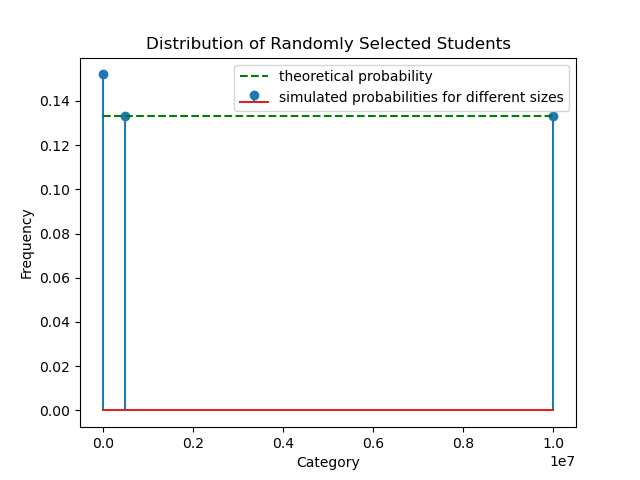
\includegraphics[width=1\columnwidth]{figures/Figure_1.png}
   \label{graph of the function}
\end{figure}

\end{document}


